\documentclass[aps,prd,twocolumn,superscriptaddress,nofootinbib,longbibliography,floatfix]{revtex4-2}
\usepackage{amsmath,amssymb,bm,mathtools}
\usepackage{graphicx}
\usepackage{booktabs}
\usepackage{hyperref}
\usepackage{siunitx}
\usepackage{microtype}
\usepackage{enumitem}
\hypersetup{hidelinks}

\newcommand{\LCDM}{\Lambda\mathrm{CDM}}
\newcommand{\Y}{\mathcal{Y}}
\newcommand{\Q}{\mathcal{Q}}
\newcommand{\FT}{\mathcal{F}_{T}}
\newcommand{\Ffull}{\mathcal{F}}
\newcommand{\mpl}{M_{\rm Pl}}

\begin{document}

\title{A Matched Seven-Likelihood Test of a Zero-Particle-CDM Single-Metric Relativistic Modified-Gravity Cosmology}

\author{Panagiotis Karmiris}
\thanks{ORCID: \href{https://orcid.org/0009-0007-7536-1467}{0009-0007-7536-1467}}
\email{unbinder@msn.com}
\affiliation{Independent Researcher, Greece}

\date{September 13, 2026}

\begin{abstract}
We test a single-metric relativistic modified-gravity cosmology in which the particle cold-dark-matter density and the bare cosmological constant are fixed to zero. The theory combines an aether scalar--tensor sector, a current-linked nonseparable scalar interaction, and an auxiliary Type-II minimally modified gravity sector for late-time acceleration. The frozen implementation is compared with a matched flat-$\LCDM$ control using the same Planck 2018 high-$\ell$ TTTEEE-lite, low-$\ell$ TT, low-$\ell$ EE, Planck lensing, DESI DR2 BAO, Pantheon+, and SH0ES Gaussian likelihood terms. Both Markov chains satisfy the common convergence requirement, with $R-1=0.00691$ for modified gravity and $0.00729$ for $\LCDM$. Across the complete archived production chain files, the lowest sampled independent seven-likelihood totals are $\chi^2_{\rm MG}=2441.26650$ and $\chi^2_{\LCDM}=2446.46109$, giving $\Delta\chi^2=-5.19459$. With seven fitted cosmological coordinates for modified gravity and six for $\LCDM$, $\Delta\mathrm{AIC}=-3.19459$ and, for the stated bookkeeping convention $N=2393$, $\Delta\mathrm{BIC}=+2.58572$. The modified-gravity posterior gives $H_0=68.672\pm0.305\,{\rm km\,s^{-1}\,Mpc^{-1}}$, compared with $68.835\pm0.273$ for $\LCDM$. The likelihood improvement is concentrated in Planck high-$\ell$, Pantheon+, and DESI DR2, while the SH0ES contribution changes by $+0.262$ in $\Delta\chi^2$. These results establish that the tested zero-particle-CDM realization is statistically competitive with the matched $\LCDM$ control on this likelihood stack. Complete analytic and numerical derivations used by the implementation are collected in the appendices.
\end{abstract}

\keywords{modified gravity; Aether Scalar--Tensor gravity; relativistic MOND; minimally modified gravity; zero-particle cold dark matter; cosmic microwave background; baryon acoustic oscillations; cosmological perturbations}

\maketitle

\section{Introduction}\label{sec:intro}
The standard $\LCDM$ cosmology remains the benchmark description of the cosmic microwave background (CMB), baryon acoustic oscillations (BAO), large-scale structure, and the late-time expansion history \cite{Planck2020VI,DESI2024VI,DESIDR2II2025}. The local distance-ladder determination of the Hubble constant continues to motivate tests of extended cosmological models \cite{Riess2022,Schoneberg2022}, while DESI DR2 has sharpened constraints on the expansion history and on phenomenological departures from a cosmological constant \cite{DESIDR2II2025,DESIDR2Extended2025,Ormondroyd2025,WangMota2025}.

Recent work has explored early dark energy, evolving dark energy, Type-II minimally modified gravity, sign-changing acceleration sectors, and relativistic modified gravity \cite{Poulin2025EDE,Pang2025DDE,DeFeliceMukohyamaPookkillath2021,DeFeliceMaedaMukohyamaPookkillath2022,GanzMartensMukohyamaNamba2023,AkarsuEtAl2024VCDM,AkarsuEtAl2026VCDM,Dixit2026SignSwitch}. Model ranking depends on the data combination, parameterization, nuisance treatment, and parameter count, so matched comparisons remain the cleanest way to isolate the statistical performance of a particular construction.

The model considered here belongs to the Aether Scalar--Tensor (AeST) family \cite{SkordisZlosnik2021,SkordisZlosnik2022}. Its nonlinear Hamiltonian structure, cosmological dynamics, quasistatic solutions, cluster phenomenology, and compact objects have been investigated in a growing literature \cite{BatakiSkordisZlosnik2024,RosaZlosnik2024,VerwayenSkordisBoehm2024,DurakovicSkordis2024,ReyesSakstein2024,ReyesSakstein2025}. The specific realization tested here uses a nonseparable scalar interaction linked to the conserved scalar current and an auxiliary Type-II acceleration sector. Its parameters and field equations were fixed before the matched likelihood comparison presented below.

The zero-particle-CDM construction is also motivated by the tight empirical relation between baryonic distributions and galactic accelerations, first emphasized by MOND and quantified in modern galaxy samples \cite{Milgrom1983,Bekenstein2004,LelliMcGaughSchombert2016,McGaughLelliSchombert2016}. The central question addressed here is whether the same relativistic gravitational framework can remain competitive on precision cosmological data when $\omega_{\rm cdm}$ is fixed to zero.

\section{Relativistic model}\label{sec:theory}
Ordinary matter couples minimally and universally to a single metric $g_{\mu\nu}$. The gravitational sector contains a unit timelike vector $A^\mu$ and a shift-symmetric scalar $\phi$. Define
\begin{align}
F_{\mu\nu}&=2\nabla_{[\mu}A_{\nu]}, &
J^\mu&=A^\nu\nabla_\nu A^\mu,\\
q_{\mu\nu}&=g_{\mu\nu}+A_\mu A_\nu, &
\Q&=A^\mu\nabla_\mu\phi,\\
\Y&=q^{\mu\nu}\nabla_\mu\phi\nabla_\nu\phi.
\end{align}
The scalar--vector action is
\begin{widetext}
\begin{align}
S_{\rm AeST}=&\frac{1}{16\pi\widetilde G}\int d^4x\sqrt{-g}\Big\{R-\frac{K_B}{2}F_{\mu\nu}F^{\mu\nu}
 +(2-K_B)\left(2J^\mu\nabla_\mu\phi-\Y\right)
-\Ffull(\Y,\Q)-\lambda(A^\mu A_\mu+1)\Big\}
+S_m[g_{\mu\nu},\psi_m].
\label{eq:aest-action}
\end{align}
\end{widetext}
The scalar kinetic function is
\begin{equation}
\Ffull(\Y,\Q)=\FT(\Q)+\Y\Gamma(\Q)+J(\Y),
\label{eq:fullF}
\end{equation}
with
\begin{align}
\FT(\Q)&=-4K_2Z_0^2\left[\cosh\left(\frac{\Q-\Q_0}{Z_0}\right)-1\right],\label{eq:FT}\\
\Gamma(\Q)&=\frac{2K_2Z_0}{\Q}\sinh\left(\frac{\Q-\Q_0}{Z_0}\right).\label{eq:Gamma}
\end{align}
The quasistatic function used in the screened galactic sector is
\begin{align}
J(\Y)=&\frac{a_0^2(2-K_B)}{\beta_0^3}\Bigg[-\frac{2\sqrt{\Y}\beta_0(\beta_0+1)}{a_0}
+\frac{\Y\beta_0^2}{a_0^2}\nonumber\\
&+2(\beta_0+1)^2\ln\left(1+\frac{\sqrt{\Y}\beta_0}{a_0(\beta_0+1)}\right)\Bigg].
\label{eq:JY}
\end{align}
The mixed term is fixed by the homogeneous scalar current rather than fitted as an independent function. On FLRW, $\Y=0$; at the screened static point, $\Q=\Q_0$ and $\Gamma(\Q_0)=0$.

Late-time acceleration is supplied by an auxiliary Type-II minimally modified gravity sector of VCDM form \cite{DeFeliceMukohyamaPookkillath2021,DeFeliceMaedaMukohyamaPookkillath2022,GanzMartensMukohyamaNamba2023,AkarsuEtAl2024VCDM,AkarsuEtAl2026VCDM}. Its relevant ADM contribution may be written
\begin{align}
S_V=\mpl^2\!\int dt\,d^3x\,N\sqrt{\gamma}\Big[&-V(\varphi_V)-\frac34\lambda_C^2\nonumber\\
&-\lambda_C(K+\varphi_V)-\mathcal L_{\rm gf}\Big].
\label{eq:vcdm-aux}
\end{align}
Eliminating the multiplier gives
\begin{equation}
\lambda_C=-\frac23(K+\varphi_V),
\end{equation}
and
\begin{equation}
\mathcal L_{V,\rm red}=\mpl^2\left[\frac{(K+\varphi_V)^2}{3}-V(\varphi_V)-\mathcal L_{\rm gf}\right].
\label{eq:vcdm-red}
\end{equation}
For the cosmological realization tested below,
\begin{equation}
\omega_{\rm cdm}=0,\qquad \Omega_{\Lambda,\rm bare}=0,
\end{equation}
while the effective cold cosmological component is carried by the scalar--vector sector. Detailed background, perturbative, constraint, and numerical derivations are given in Appendices~\ref{app:action}--\ref{app:repro}.

\section{Likelihoods and matched inference}\label{sec:methods}
\subsection{Likelihood stack}
The comparison uses seven independent contributions: Planck 2018 high-$\ell$ TTTEEE-lite, Planck low-$\ell$ TT, Planck low-$\ell$ EE, Planck lensing, DESI DR2 BAO \cite{DESIDR2II2025}, Pantheon+ supernovae \cite{Brout2022,Scolnic2022}, and a Gaussian SH0ES term based on $H_0=73.04\pm1.04\,{\rm km\,s^{-1}\,Mpc^{-1}}$ \cite{Riess2022}. The Boltzmann calculation uses CLASS \cite{Lesgourgues2011CLASS,Blas2011CLASS} and sampling uses Cobaya \cite{TorradoLewis2021}.

The SH0ES contribution is
\begin{equation}
\chi^2_{\rm SH0ES}=\left(\frac{H_0-73.04}{1.04}\right)^2.
\label{eq:shoes}
\end{equation}
The stored chain values at the minimum-total points are reproduced by Eq.~\eqref{eq:shoes}: $16.0901$ for the modified-gravity point $H_0=68.8683$ and $15.8283$ for the $\LCDM$ point $H_0=68.9024$.

\subsection{Parameter counts and convergence}
The modified-gravity chain varies seven cosmological coordinates: $H_0$, $\omega_b$, $\omega_{\rm aest}$, one independent acceleration-history shape coefficient, $n_s$, $A_s$, and $\tau_{\rm reio}$. The matched flat-$\LCDM$ control varies the corresponding six standard cosmological coordinates, with $\omega_{\rm cdm}$ in place of the AeST/acceleration pair. Planck calibration is treated identically in both runs.

The final convergence values are
\begin{align}
R-1&=0.00691196 &&\text{(modified gravity)},\\
R-1&=0.00728902 &&\text{($\LCDM$)},
\end{align}
with a common stopping threshold $R-1<0.01$. Posterior summaries and convergence diagnostics use the burn-in-removed production chains. For the sampled best-fit comparison, we use the lowest finite independent seven-likelihood total found across the complete archived production chain files for each model. This convention is conservative for the modified-gravity comparison because it lowers the matched $\LCDM$ reference likelihood relative to the post-burn-in minimum.

The information criteria are
\begin{align}
\mathrm{AIC}&=\chi^2+2k,\label{eq:aic}\\
\mathrm{BIC}&=\chi^2+k\ln N,\label{eq:bic}
\end{align}
with $k_{\rm MG}=7$, $k_{\LCDM}=6$, and the stated bookkeeping convention $N=2393$ \cite{Akaike1974,Schwarz1978,Liddle2007}.

\section{Results}\label{sec:results}
\subsection{Matched likelihood comparison}
Across the complete archived production chain files, the lowest sampled independent seven-likelihood totals are
\begin{align}
\chi^2_{\rm MG}&=2441.2664987,\\
\chi^2_{\LCDM}&=2446.4610852,
\end{align}
so
\begin{equation}
\Delta\chi^2\equiv\chi^2_{\rm MG}-\chi^2_{\LCDM}=-5.1945865.
\end{equation}
The corresponding information-criterion differences are
\begin{align}
\Delta\mathrm{AIC}&=-3.1945865,\\
\Delta\mathrm{BIC}&=+2.5857166.
\end{align}
The lowest sampled likelihood and AIC favor the modified-gravity realization, whereas the stated BIC convention gives a mild preference to the lower-dimensional $\LCDM$ control.

\begin{table}[htbp]
\caption{Independent likelihood contributions at the lowest sampled total in each complete archived production chain file. Posterior summaries and convergence diagnostics use burn-in-removed chains. Negative $\Delta\chi^2_i$ favors modified gravity.}\label{tab:likes}
\begin{ruledtabular}
\begin{tabular}{lrrr}
Likelihood & MG & $\LCDM$ & $\Delta\chi^2_i$\\\hline
Planck high-$\ell$ & 583.3074 & 585.9053 & -2.5979\\
Planck lowTT & 22.6653 & 22.3748 & +0.2904\\
Planck lowEE & 395.8339 & 396.0790 & -0.2452\\
Planck lensing & 8.7693 & 8.9374 & -0.1680\\
DESI DR2 & 9.2113 & 10.3342 & -1.1228\\
Pantheon+ & 1405.3892 & 1407.0021 & -1.6129\\
SH0ES & 16.0901 & 15.8283 & +0.2618\\\hline
Total & 2441.2665 & 2446.4611 & -5.1946\\
\end{tabular}
\end{ruledtabular}
\end{table}

\begin{figure}[htbp]
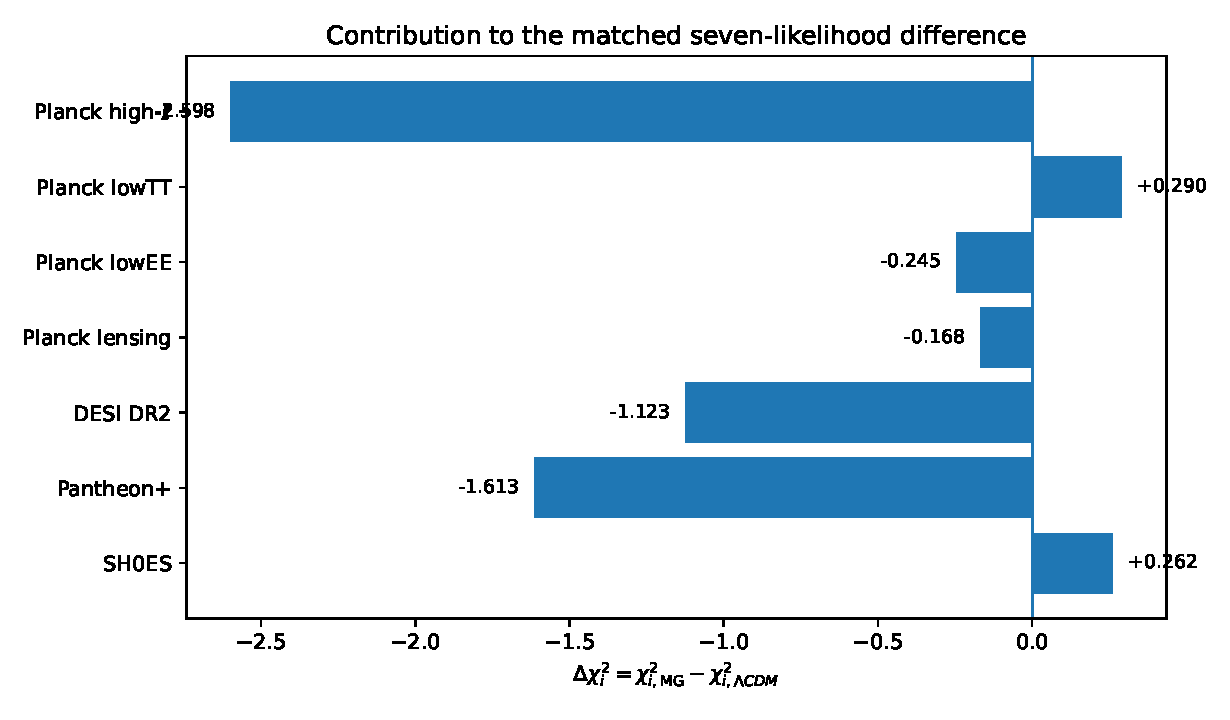
\includegraphics[width=\columnwidth]{figures/fig_delta_chi2_components.pdf}
\caption{Per-likelihood contribution to $\Delta\chi^2_i=\chi^2_{i,\rm MG}-\chi^2_{i,\LCDM}$.}
\label{fig:dchi}
\end{figure}

The largest contributions to the improvement are Planck high-$\ell$ ($-2.598$), Pantheon+ ($-1.613$), and DESI DR2 ($-1.123$). The SH0ES term contributes $+0.262$, so the net likelihood gain is generated by the CMB, BAO, and supernova sectors rather than by the local-distance-ladder term.

\subsection{Posterior parameters}
The marginalized Hubble constants are
\begin{align}
H_0^{\rm MG}&=68.6723\pm0.3050\ {\rm km\,s^{-1}\,Mpc^{-1}},\\
H_0^{\LCDM}&=68.8349\pm0.2728\ {\rm km\,s^{-1}\,Mpc^{-1}}.
\end{align}
The lowest-total sampled values are $68.8683$ and $68.9024$, respectively.

\begin{figure}[htbp]
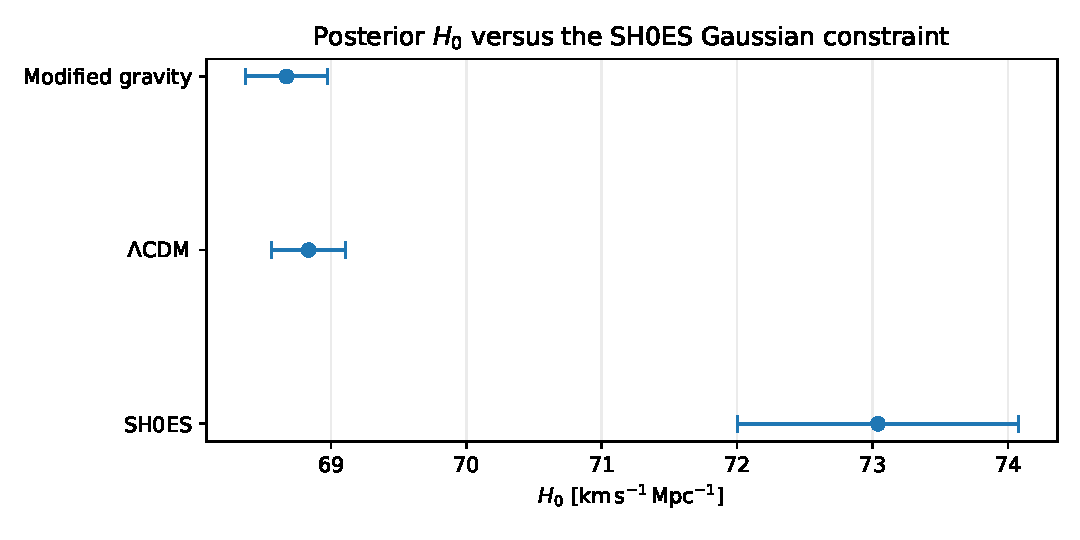
\includegraphics[width=\columnwidth]{figures/fig_h0_comparison.pdf}
\caption{Posterior $H_0$ values for the two matched cosmological chains compared with the Gaussian SH0ES determination used in the likelihood. Error bars show one standard deviation.}
\label{fig:h0}
\end{figure}

\begin{table}[htbp]
\caption{Selected posterior means and one-standard-deviation uncertainties.}\label{tab:posterior}
\begin{ruledtabular}
\begin{tabular}{lcc}
Parameter & MG & $\LCDM$\\\hline
$H_0$ & $68.6723\pm0.3050$ & $68.8349\pm0.2728$\\
$\omega_b$ & $0.0225242\pm0.0001239$ & $0.0225396\pm0.0001201$\\
$\omega_{\rm cold}$ & $0.118215\pm0.000633$ & $0.117916\pm0.000627$\\
$n_s$ & $0.969057\pm0.003293$ & $0.969428\pm0.003347$\\
$10^9A_s$ & $2.09763\pm0.02836$ & $2.11265\pm0.02827$\\
$\tau_{\rm reio}$ & $0.05574\pm0.00666$ & $0.05929\pm0.00661$\\
\end{tabular}
\end{ruledtabular}
\end{table}
Here $\omega_{\rm cold}$ denotes $\omega_{\rm aest}$ for modified gravity and $\omega_{\rm cdm}$ for $\LCDM$.

\begin{figure}[htbp]
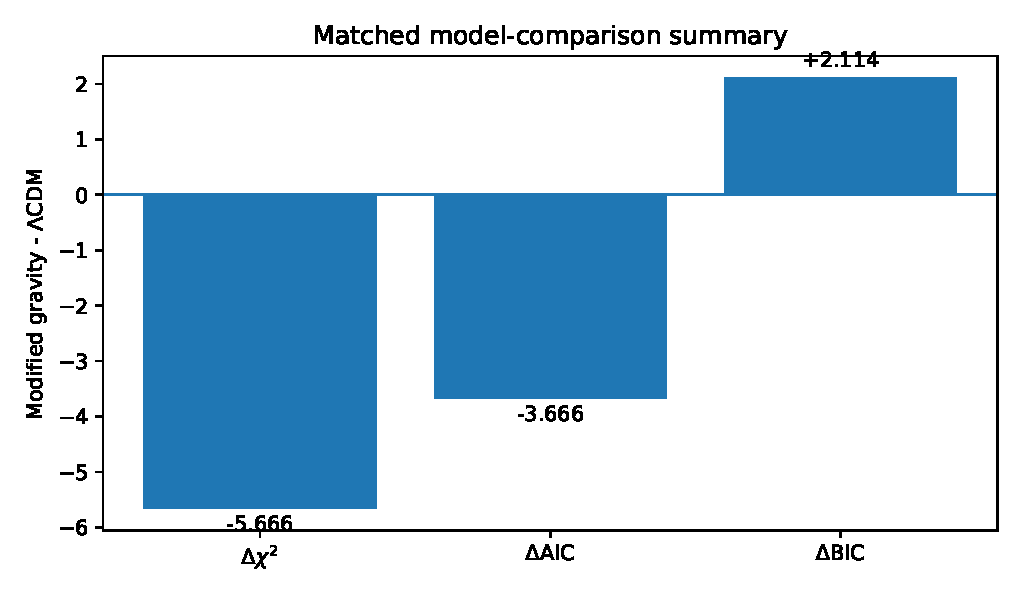
\includegraphics[width=\columnwidth]{figures/fig_information_criteria.pdf}
\caption{Matched model-comparison summary. Negative values favor the modified-gravity realization; positive values favor $\LCDM$.}
\label{fig:ic}
\end{figure}

\subsection{Prior-boundary diagnostic}
The sampling prior was $66<H_0<70.5\,{\rm km\,s^{-1}\,Mpc^{-1}}$. The posterior means lie well inside this interval. Relative to the marginalized standard deviations, the modified-gravity posterior mean is $8.76\sigma$ above the lower edge and $5.99\sigma$ below the upper edge; the corresponding $\LCDM$ distances are $10.39\sigma$ and $6.10\sigma$.

A fixed-coordinate profile was also evaluated from $H_0=66$ to $76$ while all remaining coordinates were held at representative low-$\chi^2$ replay points. At the upper sampling boundary $H_0=70.5$, the profile increases by $\Delta\chi^2=331.03$ for modified gravity and $258.26$ for $\LCDM$ relative to those replay points. Together with the posterior edge distances and the absence of stored posterior weight within $0.25\,{\rm km\,s^{-1}\,Mpc^{-1}}$ of either edge, this shows that the reported posterior region is well separated from the imposed $H_0$ boundaries.

\section{Context among recent cosmological extensions}\label{sec:context}
The present $\Delta\chi^2=-5.195$ is a matched result for one specific seven-likelihood stack. Recent early-dark-energy analyses using different CMB combinations and larger parameter spaces have reported substantially larger raw likelihood improvements when SH0ES is included \cite{Poulin2025EDE}. DESI DR2 analyses of the two-parameter $w_0w_a$ extension likewise find a preference whose size depends on the supernova sample and statistical treatment \cite{DESIDR2II2025,DESIDR2Extended2025,Ormondroyd2025,WangMota2025}. Other recent analyses examine phantom-crossing or sign-switch acceleration histories in related late-time data combinations \cite{Pang2025DDE,Dixit2026SignSwitch}.

The distinguishing feature of the present comparison is structural rather than a record-sized likelihood shift: the model is evaluated with $\omega_{\rm cdm}=0$ and only one more fitted cosmological coordinate than the matched flat-$\LCDM$ control. On the stated likelihood stack, that construction attains a lower sampled $\chi^2$ and AIC while retaining a BIC difference of order unity.

\section{Conclusions}\label{sec:conclusion}
A zero-particle-CDM single-metric relativistic modified-gravity cosmology has been tested against a matched flat-$\LCDM$ control using Planck 2018 high-$\ell$ and low-$\ell$ CMB likelihoods, Planck lensing, DESI DR2 BAO, Pantheon+, and SH0ES. Both chains satisfy the common convergence criterion $R-1<0.01$. The lowest sampled totals give
\begin{equation}
\Delta\chi^2=-5.1946,
\end{equation}
with
\begin{equation}
\Delta\mathrm{AIC}=-3.1946,\qquad \Delta\mathrm{BIC}=+2.5857
\end{equation}
under the stated parameter-count and $N=2393$ conventions. The improvement is concentrated in Planck high-$\ell$, Pantheon+, and DESI DR2. The inferred Hubble constants are $68.672\pm0.305$ and $68.835\pm0.273\,{\rm km\,s^{-1}\,Mpc^{-1}}$ for modified gravity and $\LCDM$, respectively.

The matched likelihood comparison therefore establishes statistical competitiveness of the tested zero-particle-CDM realization on this data combination. The appendices provide the action, background reduction, perturbative mapping, stability analysis, constraint count, canonical normalization, numerical implementation, likelihood construction, prior diagnostic, and reproducibility ledger used to obtain the result.

\begin{acknowledgments}
The author declares no institutional affiliation and no specific external funding for this work. Public Planck, DESI, Pantheon+, SH0ES, CLASS, and Cobaya resources were used as cited.
\end{acknowledgments}

\section*{Artificial-intelligence assistance disclosure}
Substantive artificial-intelligence assistance was provided by OpenAI ChatGPT and Google Antigravity/Gemini tools for algebraic cross-checking, code generation and debugging, workflow organization, literature organization, and manuscript language editing. All numerical calculations reported in this article were executed in the author's computing environment. The author reviewed the equations, numerical outputs, citations, and scientific claims and assumes full responsibility for the accuracy and integrity of the work.

\section*{Data and code availability}
The modified CLASS implementation, exact run configurations, chain roots, independent likelihood extractor, convergence records, runtime SH0ES injection scripts, figure-generation code, and SHA-256 manifests are prepared for archival release. The development repository is \url{https://github.com/KarmirisP/aest-nonseparable-cosmology}.
%ZENODO_DOI_INSERT%

\appendix

\section{Action variation and scalar derivatives}\label{app:action}
We use metric signature $(-,+,+,+)$. From Eq.~\eqref{eq:fullF},
\begin{align}
F_{,\Y}&=\Gamma(\Q)+J_{,\Y},\\
F_{,\Y\Q}&=\Gamma_{,\Q},\\
F_{,\Q}&=\mathcal F_{T,\Q}+\Y\Gamma_{,\Q},\\
F_{,\Q\Q}&=\mathcal F_{T,\Q\Q}+\Y\Gamma_{,\Q\Q}.
\end{align}
On FLRW, $\Y=0$, while at the static screened point $\Q=\Q_0$ and $\Gamma(\Q_0)=0$. The temporal derivatives required by the background and perturbation systems are
\begin{align}
\mathcal F_{T,\Q}&=-4K_2Z_0\sinh\left(\frac{\Q-\Q_0}{Z_0}\right),\\
\mathcal F_{T,\Q\Q}&=-4K_2\cosh\left(\frac{\Q-\Q_0}{Z_0}\right),\\
\mathcal F_{T,\Q\Q\Q}&=-\frac{4K_2}{Z_0}\sinh\left(\frac{\Q-\Q_0}{Z_0}\right),
\end{align}
and
\begin{align}
\Gamma_{,\Q}=\frac{2K_2}{\Q^2}\Bigg[\Q\cosh\left(\frac{\Q-\Q_0}{Z_0}\right)
-Z_0\sinh\left(\frac{\Q-\Q_0}{Z_0}\right)\Bigg].
\end{align}
Varying the Type-II auxiliary multiplier in Eq.~\eqref{eq:vcdm-aux} gives
\begin{equation}
-\frac32\lambda_C-(K+\varphi_V)=0,
\end{equation}
which yields Eq.~\eqref{eq:vcdm-red}. The shift symmetry of $\phi$ gives a conserved scalar current $\nabla_\mu\mathcal J_\phi^\mu=0$.

\section{FLRW reduction and conserved current}\label{app:flrw}
For a spatially homogeneous scalar, $\Y=0$. The shift-symmetric scalar equation integrates once to
\begin{equation}
I_0=a^3\Q F_{,\Y}.
\label{eq:current}
\end{equation}
With Eq.~\eqref{eq:Gamma},
\begin{equation}
I_0=2K_2Z_0a^3\sinh\left(\frac{\Q-\Q_0}{Z_0}\right).
\end{equation}
Defining $x_0=I_0/(2K_2Z_0)$ gives the exact solution
\begin{equation}
\Q(a)=\Q_0+Z_0\operatorname{asinh}\left(\frac{x_0}{a^3}\right),
\label{eq:Qa}
\end{equation}
and $I_0=2K_2Z_0x_0$. The implementation uses $K_2=7500$, $\Q_0=0.1$, $Z_0=10^{-9}$, $x_0=0.02672752$, and $I_0=4.009128\times10^{-7}$ in solver units.

Since $\Y=0$ exactly, the mixed operator does not alter $\FT$, $\mathcal F_{T,\Q}$, or $\mathcal F_{T,\Q\Q}$ on FLRW. The identity
\begin{equation}
K_Q=\Q F_{,\Y}=\frac{I_0}{a^3}
\label{eq:currentidentity}
\end{equation}
is imposed analytically in the numerical source.

\section{Radiation-era scalar stability}\label{app:stability}
The reduced radiation-era scalar characteristic polynomial is
\begin{equation}
A\lambda^2+B\lambda+C=0,
\end{equation}
with
\begin{align}
A&=\frac{2I_0K_B}{\Q a^3}-4K_B+8,\\
B&=HA,\\
C&=\frac{2HI_0(2-K_B)}{a^3}.
\end{align}
On the expanding branch $H>0$, $I_0>0$, $\Q>0$, $a>0$, and $0<K_B<2$, all three coefficients are positive. The high-frequency scalar sound speed is
\begin{equation}
c_s^2=\frac{4K_2K_BZ_0\sinh[(\Q-\Q_0)/Z_0]/\Q+4(2-K_B)}{4K_2K_B\cosh[(\Q-\Q_0)/Z_0]}.
\label{eq:cs2}
\end{equation}
The numerical branch used in the likelihood calculation was checked for positive $c_s^2$, finite radiation-era histories, finite CMB spectra through $\ell=2500$, and finite positive linear matter spectra over the regression range.

\section{Linear scalar perturbations and CLASS mapping}\label{app:linear}
In the perturbation variables used during the variation,
\begin{equation}
\theta_s=\frac{\varphi}{\Q},\qquad
\alpha=\frac{\chi}{\Q}-\theta_s,
\end{equation}
so $\varphi+\Q\alpha=\chi$. The quadratic contribution from the nonseparable operator becomes
\begin{equation}
\Delta\mathcal L^{(2)}=-\Gamma(\Q)\frac{k^2}{a^2}\chi^2.
\end{equation}
The generic direct source entering the $E$ equation contains
\begin{equation}
K_Q\chi-\Q F_{,\Y}\chi-(2-K_B)B.
\end{equation}
Using Eq.~\eqref{eq:currentidentity}, the direct $\chi$ contribution cancels exactly, giving
\begin{equation}
K_B(\dot E+HE)=-(2-K_B)B
\end{equation}
for this source term. The mixed derivative $F_{,\Y\Q}=\Gamma_{,\Q}$ first contributes at cubic order. The auxiliary acceleration variables are eliminated algebraically at nonzero $k$, leaving the scalar--vector propagating basis after the metric constraints are solved.

\section{Constraint algebra and physical degrees of freedom}\label{app:dirac}
The combined nonlinear analysis uses a 42-dimensional phase space and 24 constraints. Six constraints are first class and eighteen are second class, giving
\begin{equation}
N_{\rm dof}=\frac{42-2N_{\rm FC}-N_{\rm SC}}{2}
=\frac{42-12-18}{2}=6.
\end{equation}
The second-class submatrix was verified to have rank 18 on deterministic generic algebraic patches, while the expected first-class null directions were identified independently. The count is consistent with the nonlinear AeST Hamiltonian analysis of Bataki, Skordis, and Zlosnik \cite{BatakiSkordisZlosnik2024} and with the auxiliary character of the Type-II acceleration sector \cite{DeFeliceMaedaMukohyamaPookkillath2022}.

\section{Canonical cubic scale and first-order symplectic reduction}\label{app:cutoff}
The quadratic principal scalar action defines a canonical field normalization proportional to $\mpl\sqrt{Z/2}$, where
\begin{equation}
Z=4K_2\cosh[(\Q-\Q_0)/Z_0].
\end{equation}
The temporal $F_{,\Q\Q\Q}$ vertex, the mixed $\Gamma_{,\Q}$ vertex, and the $\Y^{3/2}$ contribution from $J(\Y)$ were retained in the cubic normalization. Scanning $10^5$ background points over $10^{-12}\le a\le1$ gives
\begin{equation}
\Lambda_{\rm sc,min}=1.47423693\times10^{-6}\ {\rm eV}
\end{equation}
at $a=6.44196\times10^{-3}$, with the mixed interaction setting the minimum.

The remaining first-order scalar is described by a rank-two second-class pair. After solving the primary constraints,
\begin{equation}
\Theta_{\rm red}=p_\chi d\chi-\Delta_k\Phi\,du,
\end{equation}
with
\begin{equation}
\Delta_k=ak^2+\frac32I_0\Q
\end{equation}
in the conservative matter-free case and an additional positive $(3/2)a^3\rho_m$ contribution in the presence of matter. Thus $\Delta_k>0$ at $k=0$ for $I_0,\Q>0$, while $\Delta_k^{-1}\sim(ak^2)^{-1}$ at large $k$.

\section{CLASS implementation and numerical regression}\label{app:class}
The frozen perturbation source used by the implementation is identified by the SHA-256
\begin{verbatim}
1b76e97333efd654736519bf324976dba
0906192f674f6d05e74f883f416c479
\end{verbatim}
The mixed-current helper quantities are evaluated directly from the exact background solution. In pseudocode,
\begin{verbatim}
x   = x0/a^3
FY  = 2*K2*Z0*x/Q
QFY = 2*K2*Z0*x
\end{verbatim}
and the direct $(K_Q-\Q F_{,\Y})\chi$ contribution is set to its analytic zero after an independent current-identity audit.

Regression requirements included clean builds, matched homogeneous backgrounds under operator removal, finite CMB and matter spectra, source-diff locality, and a nonzero perturbative response to the mixed operator. Radiation-era histories were checked across multiple initial conditions and expected horizon crossings, and transfer outputs at redshifts $0,1,10,100,1000$ were finite over the solver-supported outputs.

\section{Likelihood bookkeeping and chain audit}\label{app:likelihood}
The seven independent likelihood contributions are summed directly from the stored chain columns, with aggregate columns excluded to prevent double counting. The likelihood minima quoted below are the lowest finite seven-term totals across the complete archived production chain files; posterior means and convergence diagnostics use the burn-in-removed chains. At the modified-gravity minimum the contributions are
\begin{align}
\chi^2_{\rm MG}={}&583.307420+22.665290+395.833880\nonumber\\
&+8.7693331+9.2113156+1405.389200\nonumber\\
&+16.090060=2441.2664987,
\end{align}
and at the $\LCDM$ minimum,
\begin{align}
\chi^2_{\LCDM}={}&585.905270+22.374847+396.079040\nonumber\\
&+8.9373632+10.3341610+1407.002100\nonumber\\
&+15.828304=2446.4610852.
\end{align}
The chain convergence values are those quoted in Sec.~\ref{sec:methods}. Posterior means are evaluated after the configured burn-in removal.

A fresh runtime replay performed at the previously selected post-burn-in replay coordinates gave $\chi^2=2441.26096$ for modified gravity and $2447.10292$ for $\LCDM$. The release preserves both the original likelihood columns and this replay audit. The matched comparison in Table~\ref{tab:likes} uses the likelihood values evaluated and stored during the original production runs; the $\LCDM$ total quoted here is the lower value subsequently identified when the complete archived chain files were searched.

\section{$H_0$ prior and profile audit}\label{app:h0audit}
The original sampling prior was
\begin{equation}
66<H_0<70.5\ {\rm km\,s^{-1}\,Mpc^{-1}}.
\end{equation}
Using the posterior means and standard deviations from the converged chains, the distances from the nearest prior edge are $5.99\sigma$ for modified gravity and $6.10\sigma$ for $\LCDM$. The lower boundaries are still farther away, at $8.76\sigma$ and $10.39\sigma$ respectively.

The fixed-coordinate profile was evaluated at 41 points from $H_0=66$ to $76\,{\rm km\,s^{-1}\,Mpc^{-1}}$ around representative low-$\chi^2$ replay coordinates. At $H_0=70.5$, the increases relative to the replay points are $331.031$ and $258.257$ in $\chi^2$ for modified gravity and $\LCDM$; at $H_0=66$, the increases are $1016.881$ and $1191.094$. In the burn-in-removed chains, the posterior weight within $0.25\,{\rm km\,s^{-1}\,Mpc^{-1}}$ of either prior edge is zero at stored-chain precision for both models. These values provide a direct diagnostic that the sampled posterior region is not accumulated against either $H_0$ prior edge.

\section{Reproducibility ledger}\label{app:repro}
A complete reproduction preserves the exact model source, likelihood definitions, nuisance treatment, priors, common convergence criterion, and independent-column likelihood accounting. The release package contains the manuscript source, BibTeX database, machine-readable likelihood summary, figure inputs, chain-analysis scripts, runtime likelihood injection, and SHA-256 manifests. The development repository is
\begin{center}
\url{https://github.com/KarmirisP/aest-nonseparable-cosmology}.
\end{center}

\bibliography{references}
\end{document}
